\pgfdeclarelayer{background}
\pgfsetlayers{background,main}
\def\scale{1.5}

\colorlet{circle edge}{black!50}
\colorlet{circle area}{gray!20}

\tikzset{
  filled/.style={fill=circle area, draw=circle edge, thick},
  outline/.style={draw=circle edge, thick}
  }

\setlength{\parskip}{5mm}

\tikzstyle{edge} = [draw, thick,-]
\tikzstyle{stribe} = [draw, dashed,-]
\tikzstyle{vertex}=[circle,fill=black!25,minimum size=10pt,inner sep=0pt]
\tikzstyle{black vertex}=[circle, fill=black!100,minimum size=10pt, inner sep=0pt]
\tikzstyle{invis-vertex}=[circle,fill=white!100,minimum size=0pt, inner sep=0pt]

\tikzstyle{greedy edge} = [draw,line width=5pt,-,gray!50]
\tikzstyle{perimiter edge} = [draw,line width=5pt,-,black!100]

\def\sinkSource{{(0, 0)/s}, {(5.4, 2)/t}}
\def\normalNodes{{(3.25, 2)/h}, {(2.3, 2.2)/k}, {(1.7, 2.3)/l}, {(1.34, 1.7)/m}, {(1.6, 1.6)/n}, {(1.4, 1.3)/o}, {(4.1, 2.5)/z}, {(3.8, 1.8)/a1}, {(5.3, 2.6)/e1}, {(4.9, 2.6)/f1}, {(4.4, 2.65)/g1}, {(2.7, 1.2)/u}, {(2.8, 1.8)/v}}

\def\blackSpecialNodes{{(1.7, 0.65)/c}, {(1.5, 0.3)/x}, {(2, 0)/d}, {(2.4, 0.6)/e}, {(4.3, 1.6)/b1}, {(4.6, 0.9)/c1}, {(5.3, 1.1)/d1}}
\def\greySpecialNodes{{(0.5, 0.5)/a}, {(1.2, 0.89)/b}, {(2.7, 0.7)/f}, {(3.2, 1.2)/g}, {(3.5, 1.4)/q}}

\def\connect{s/a-, a-/b-, b-/c-, c-/x-, x-/d-, d-/e-, e-/f-, f-/g-, g-/q-, h-/q-, h-/v-, v-/u-, u-/f-, v-/k-, k-/l-, l-/m-, m-/n-, n-/o-, o-/c-, h-/z-, z-/a1-, a1-/b1-, b1-/q-, b1-/c1-, c1-/d1-, d1-/t, t/e1-, e1-/f1-, f1-/g1-, g1-/z-}

\def\greedy{s-/a-, a-/b-, b-/c-, e-/f-, f-/g-, g-/q-, q-/b1-, d1-/t-}
\def\perimiter{c-/x-, x-/d-, d-/e-, b1-/c1-, c1-/d1-}

\def\greedyPath{s/a, a/b, b/x}

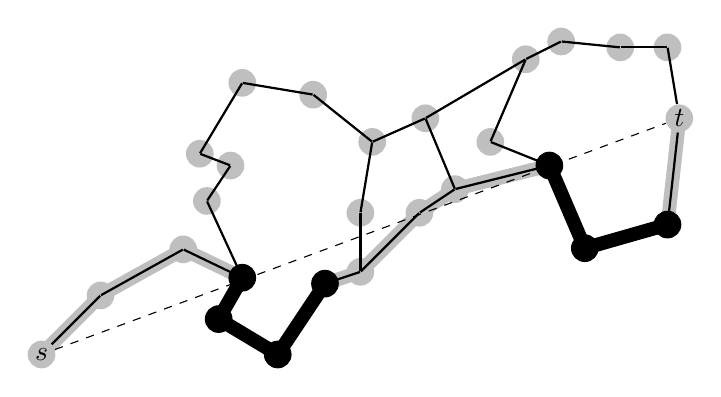
\begin{tikzpicture}[scale=\scale]

  \foreach \pos/\name in \sinkSource {
    \node[invis-vertex] (\name-) at \pos {};
    \node[vertex] (\name) at \pos {$\name$};
    }

  \foreach \pos/\name in \normalNodes {
    \node[invis-vertex] (\name-) at \pos {};
    \node[vertex] () at \pos {};
    }

  \foreach \pos/\name in \greySpecialNodes {
    \node[invis-vertex] (\name-) at \pos {};
    \node[vertex] (\name) at \pos {};
    }

  \foreach \pos/\name in \blackSpecialNodes {
    \node[invis-vertex] (\name-) at \pos {};
    \node[black vertex] (\name) at \pos {};
    }
  
  \foreach \source/\sink in \connect {
    \path[edge] (\source) -- (\sink);
    }

  \path[stribe] (s) -- (t);
  

  \begin{pgfonlayer}{background}
    \foreach \source/ \dest in \greedy
      \path[greedy edge] (\source) -- (\dest);
  
    \foreach \source/ \dest in \perimiter
      \path[perimiter edge] (\source) -- (\dest);
  \end{pgfonlayer}

\end{tikzpicture}
